\documentclass[10pt]{report}

\usepackage{talk}
\usepackage[export]{adjustbox}

\newcommand{\draw}[2]{#1^{(#2)}}
\newcommand{\displayfrac}[2]{{\displaystyle \frac{\displaystyle #1}{\displaystyle #2}}}
\newcommand{\simvar}[1]{#1^{\textrm{sim}}}
\newcommand{\simdraw}[2]{#1^{\textrm{sim}(#2)}}

\begin{document}
\sf%
\mbox{ }
\\[12pt]
\spc{\LARGE\bfseries \myemph{Bayesian Workflow}}
\\[8pt]
\spc{\LARGE\bfseries \myemph{with probabilistic programming}}
\\[36pt]
\noindent
\spc{\Large \myemph{Bob Carpenter}}
\\[4pt]
\spc{\large Center for Computational Mathematics}
\\[2pt]
\spc{\large Flatiron Institute}
\\[2pt]
\spc{\large New York}
\vfill
\noindent
\spc{\small \myemph{Netherlands eScience SIG}, October 2024} \hfill

\includegraphics[width=1in]{flatiron-logo.png}
% \mypart{}{Motivation}

\sld{Textbook form of workflow}
\begin{enumerate}
    \item Set up a \myemph{full probability model}---a joint
      distribution for observables and unobservables consistent with
      knowledge about the scientific problem and data collection.
    \item \myemph{Condition on observed data}: calculate and interpret the
      \myemph{posterior distribution}.
    \item \myemph{Evaluate the fit and implications}: does it fit
      data, are conclusions reasonable, is it sensitive to
      assumptions?
    \item \myemph{Iterate}: If model fails evaluation, go back to (1).
      \begin{subitemize}
      \item For statisticians, last two steps were \myemph{revolutionary}.
      \end{subitemize}
    \end{enumerate}
      \vfill
      \spc {\footnotesize Gelman et al. 2013.  \textit{Bayesian Data
          Analysis, 3rd Edition}. Chapman \& Hall.}
    
\sld{Bayesian workflow involves}
\begin{subitemize}
  \item \myemph{designing experiments} and \myemph{collecting data},
  \item \myemph{designing / coding} probability models,
  \item evaluating \myemph{likelihoods} and \myemph{priors},
  \item \myemph{fitting} models to data,
  \item \myemph{validating} computation,
  \item addressing \myemph{computational issues},
  \item \myemph{evaluating} and \myemph{comparing} model fit and predictions,
  \item \myemph{modifying / improving} models, and
  \item \myemph{deploying} models predictively (prospective or retrospective).
    \vfill
\end{subitemize}


\sld{A workflow chart}
\begin{center}
\vspace*{-6pt}
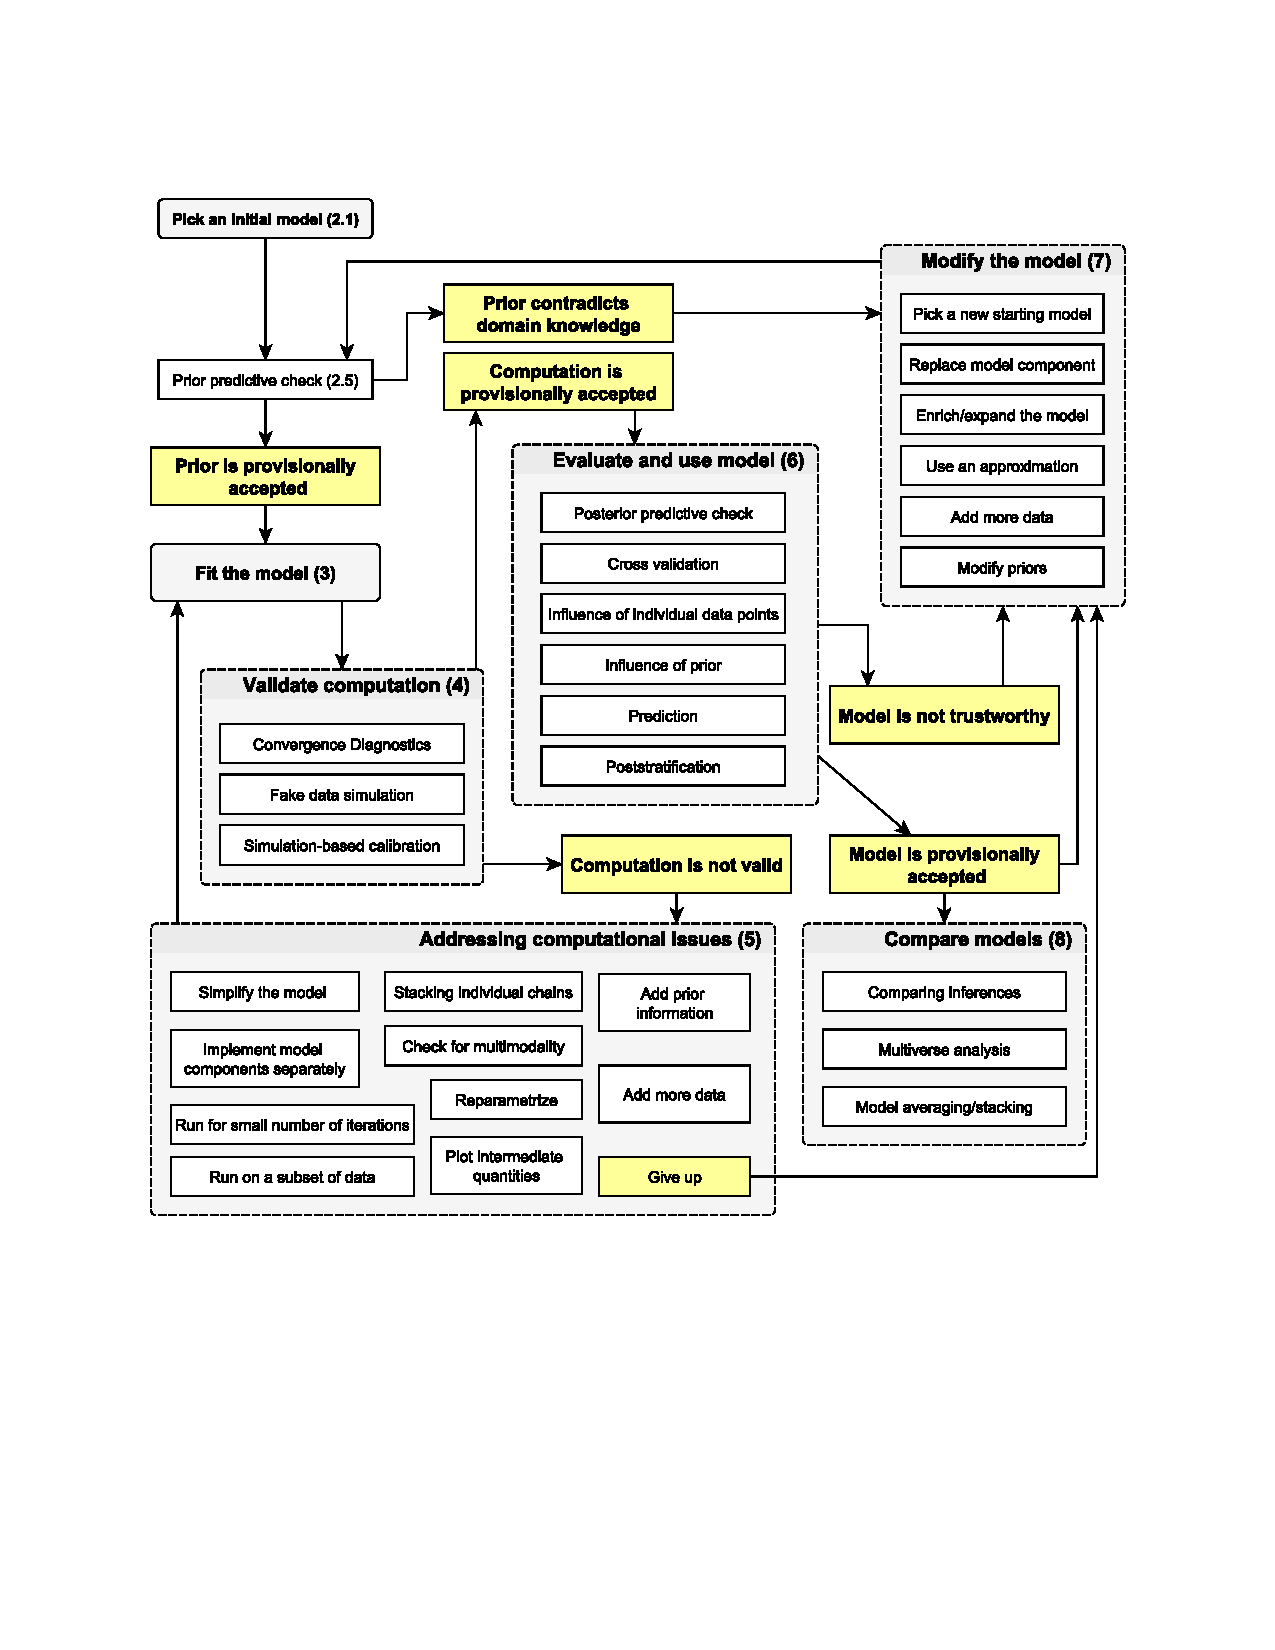
\includegraphics[height=0.85\textheight]{img/workflow-fig.pdf}
\\[-2pt]
\spc {\footnotesize Gelman et al. 2020.  Bayesian
        worflow. \textit{arXiv}.} \hfill \mbox{ }
\end{center}


\sld{Bayesian models}
\begin{itemize}
\item $y$ is \myemph{observed data}, $\theta$ are \myemph{unknown parameters}
\begin{subitemize}
\item suppress unmodeled predictors/features $x$
\end{subitemize}
\item \myemph{prior} distribution: $p(\theta)$
\item \myemph{sampling} distribution: $p(y \mid \theta)$
  \begin{subitemize}
    \item \myemph{likelihood} function: $\mathcal{L}(\theta) = p(y \mid \theta)$ for fixed $y$
  \end{subitemize}
\item \myemph{joint} distribution: $p(y, \theta) = p(y \mid \theta)\cdot p(\theta)$
\item \myemph{posterior} distribution:
  $$
  p(\theta \mid y)
  = \dfrac{p(y, \theta)}{p(y)}
  = \dfrac{p(y \mid \theta) \cdot p(\theta)}{\int p(y \mid \theta)
    \cdot p(\theta) \textrm{d}\theta}
  \propto p(y \mid \theta) \cdot p(\theta)
  $$
\end{itemize}

\sld{Prior and likelihood}
\begin{itemize}
\item The prior and likelihood can \myemph{only be understood
    together}
  \vspace*{-12pt}
  \begin{subitemize}
  \item choosing both is \myemph{subjective}, but
  \item \myemph{likelihood more important}
    \item e.g., linear in log
      odds, compartment ode model, $\ldots$
  \end{subitemize}
\item The prior represents \myemph{what you already know}
  \begin{subitemize}
    \item often just \myemph{weakly informative} to \myemph{determine
        scale}
    \end{subitemize}
  \item \myemph{Sampling distribution} encodes \myemph{data
      generating process}
    \vspace*{-12pt}
    \begin{subitemize}
    \item typically a scientific \myemph{forward model}
    \item coupled with a \myemph{noisy observation model}
    \end{subitemize}
  \end{itemize}

\sld{Estimating gravity \hfill {\normalsize (Galielo, Newton 17th c.)}}
\begin{itemize}
\item Roll balls down a ramp and \myemph{measure position vs.\ time $t$}.
\item Solve \myemph{Newton's differential equation} for expected position $\hat{y}(t)$ given (a) initial position,
  (b) slope of ramp, (c) \myemph{unknown gravitational constant} $G$, (d)
  measurement position.
\item Express \myemph{prior \slshape knowledge} as a distribution over plausible values
  of the gravitational constant: $G \sim \textrm{normal}(6.7, 0.2)$
\item Model the \myemph{measurement error} of your process
  probabilistically
  $y \sim \textrm{normal}(\hat{y}, \sigma)$.
\item Evaluate the \myemph{posterior} distribution to see what you
  \myemph{learned from data}: $p(G \mid y)$.
\end{itemize}

\sld{Science is so cool! \hfill {\normalsize Galileo Museum}}
\begin{center}
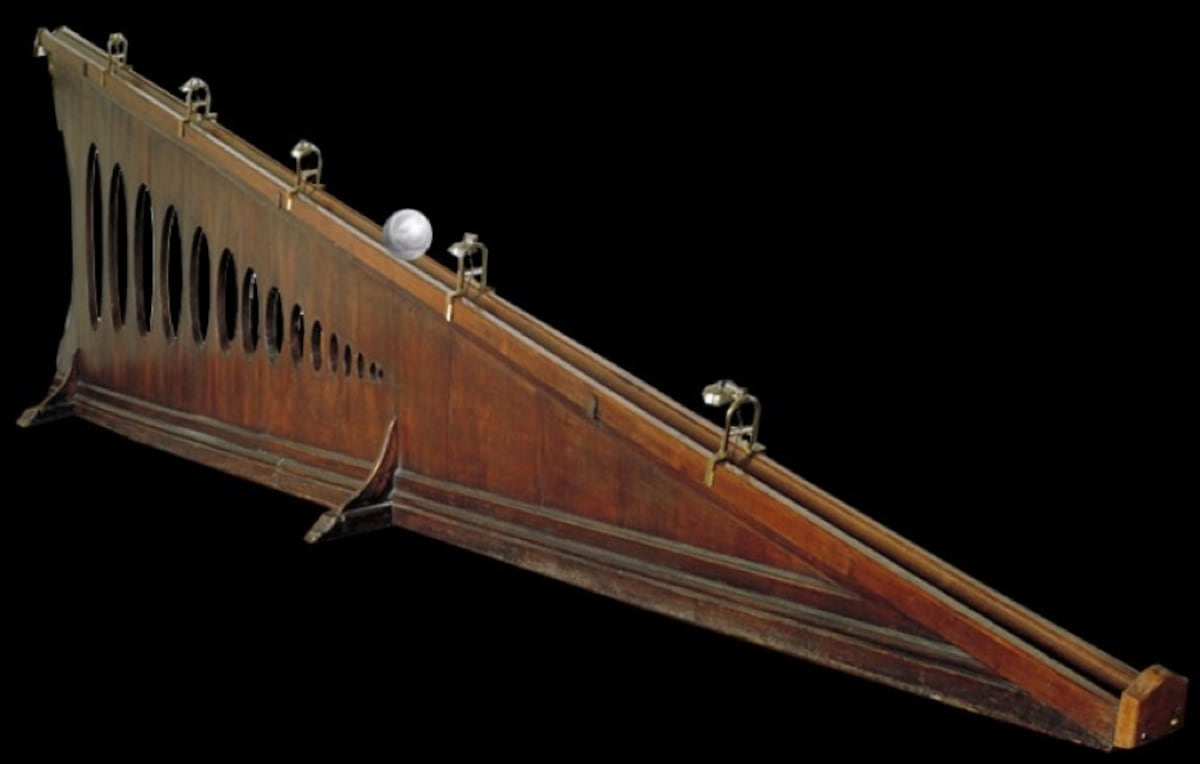
\includegraphics[width=0.9\textwidth]{galileo-plane.jpeg}
\end{center}

\sld{What makes inference Bayesian?}
\begin{itemize}
\item It's \myemph{not} the use of a prior.
\item It's \myemph{averaging over posterior uncertainty}.
\item Bayesian inference involves \myemph{posterior expectations},
  which are defined as posterior averages.
\end{itemize}

\sld{Parameter estimation}
\begin{itemize}
\item An \myemph{estimator} maps data $y$ to estimated parameter value.
\item \myemph{Bayesian parameter estimate} is posterior expectation
  $$
  \hat{\theta} = \mathbb{E}[\theta \mid y].
  $$
\item The posterior expectation is the estimate that \myemph{minimizes
    expected square error} (over random data sets),
  $$
  \hat{\theta} = \textrm{argmin}_\theta \ \mathbb{E}_{p(y)}\left[\left( \strut\theta -
      \mathbb{E}\left[\theta \mid y\right]\right)^2\right].
  $$
\item \myemph{Variance} estimates involve an expectation of $\theta^2$.
\end{itemize}
  
\sld{Event probability}
\begin{itemize}
\item An \myemph{event} $C$ is a subset of parameter space.
\item Bayesian \myemph{event probability estimate}
 $$
 \textrm{Pr}[C \mid y] = \mathbb{E}[I_C(\theta) \mid y],
  $$
  where $\textrm{I}_C(\theta) = 1$ if $\theta \in C$ and $0$ otherwise.
\item Events \myemph{can be anything},
  \begin{subitemize}
  \item e.g., $\Pr[\theta > 0.5 \mid y]$, where $\theta$ is proportion
    of male live births, for the event probability of there being more
    male live births than female (Laplace's original inference
    problem),
    with $y$ being records of male births out of total births for 50 years
    \end{subitemize}
\end{itemize}

\sld{Posterior predictive distribution}
\begin{itemize}
\item \myemph{Predicts new data} given observed data (and covariates).
\item \myemph{Posterior predictive distribution}
$$p(\tilde{y} \mid y) =
  \mathbb{E}[p(\tilde{y} \mid \theta) \mid y],
$$
where $\tilde{y}$ is \myemph{new data}, $y$ is \myemph{observed data}
\item \myemph{Averages} prediction of $\tilde{y}$ over uncertainty in $\theta$
  given $y$
\item Can \myemph{condition} everything on covariates (e.g., blood pressure,
  soil carbon concentration, distance from the moon, etc.)
\end{itemize}

\sld{Expectations via Monte Carlo}
\begin{itemize}
  \item calculate \myemph{asymptotically exact} expectations by averaging
\begin{eqnarray*}
  \mathbb{E}[f(\theta) \mid y]
  & = & \textstyle \int_{\Theta} f(\theta) \cdot p(\theta \mid y) \,
        \textrm{d}\theta
        \\[4pt]
  & = & \textstyle \lim_{M \rightarrow \infty} \frac{1}{M} \sum_{m = 1}^M
        f(\draw{\theta}{m})
        \\[4pt]
  & \approx & \textstyle \frac{1}{M} \sum_{m = 1}^M (\draw{\theta}{m}),
\end{eqnarray*}
\item MCMC \myemph{central limit theorem} says that if draws
\[
  \draw{\theta}{1}, \ldots, \draw{\theta}{M} \sim p(\theta \mid y)
\]
have \myemph{effective sample size} $M_{\textrm{eff}}$, then
\myemph{standard error} is
\[
\textrm{se}(\hat{\theta})
  = \displayfrac{\textrm{sd}[\theta \mid y]}
                {\sqrt{M_{\textrm{eff}}}} 
\]
\end{itemize}

\sld{PPLs}
\begin{itemize}
\item \myemph{Probabilistic programming languages} (PPLs)
\begin{subitemize}  
\item \myemph{code} Bayesian \myemph{joint densities} (up to
  constant), and
\item \myemph{sample} $\theta^{(n)} \sim p(\theta \mid y)$ from the
  posterior to compute expectations via Monte Carlo
\end{subitemize}
  \vfill
\item It turns out that
  \\
  we \myemph{need more than posterior sampling} for workflow.
\end{itemize}

\sld{Prior predictive checks}
\begin{itemize}
\item Prior predictive checks \myemph{simulate data} from the marginal
  \[
    \simvar{y} \sim p(y)
  \]
\item often by simulating from the \myemph{joint}, by generating from \myemph{prior} and \myemph{sampling} distributions
  \[
    \simvar{\theta} \sim p(\theta)
    \qquad
    \simvar{y} \sim p(y \mid \simvar{\theta})
  \]
\item Then \myemph{compare} simulated data $\simvar{y}$ to observed $y$
  \vfill
  {\footnotesize Gabry, Simpson, Vehtari, Betancourt,
    Gelman. 2019. Visualization in Bayesian workflow. \textit{JRSS A}.}
\end{itemize}

\sld{Prior predictive example}

\begin{center}
\vspace*{-8pt}
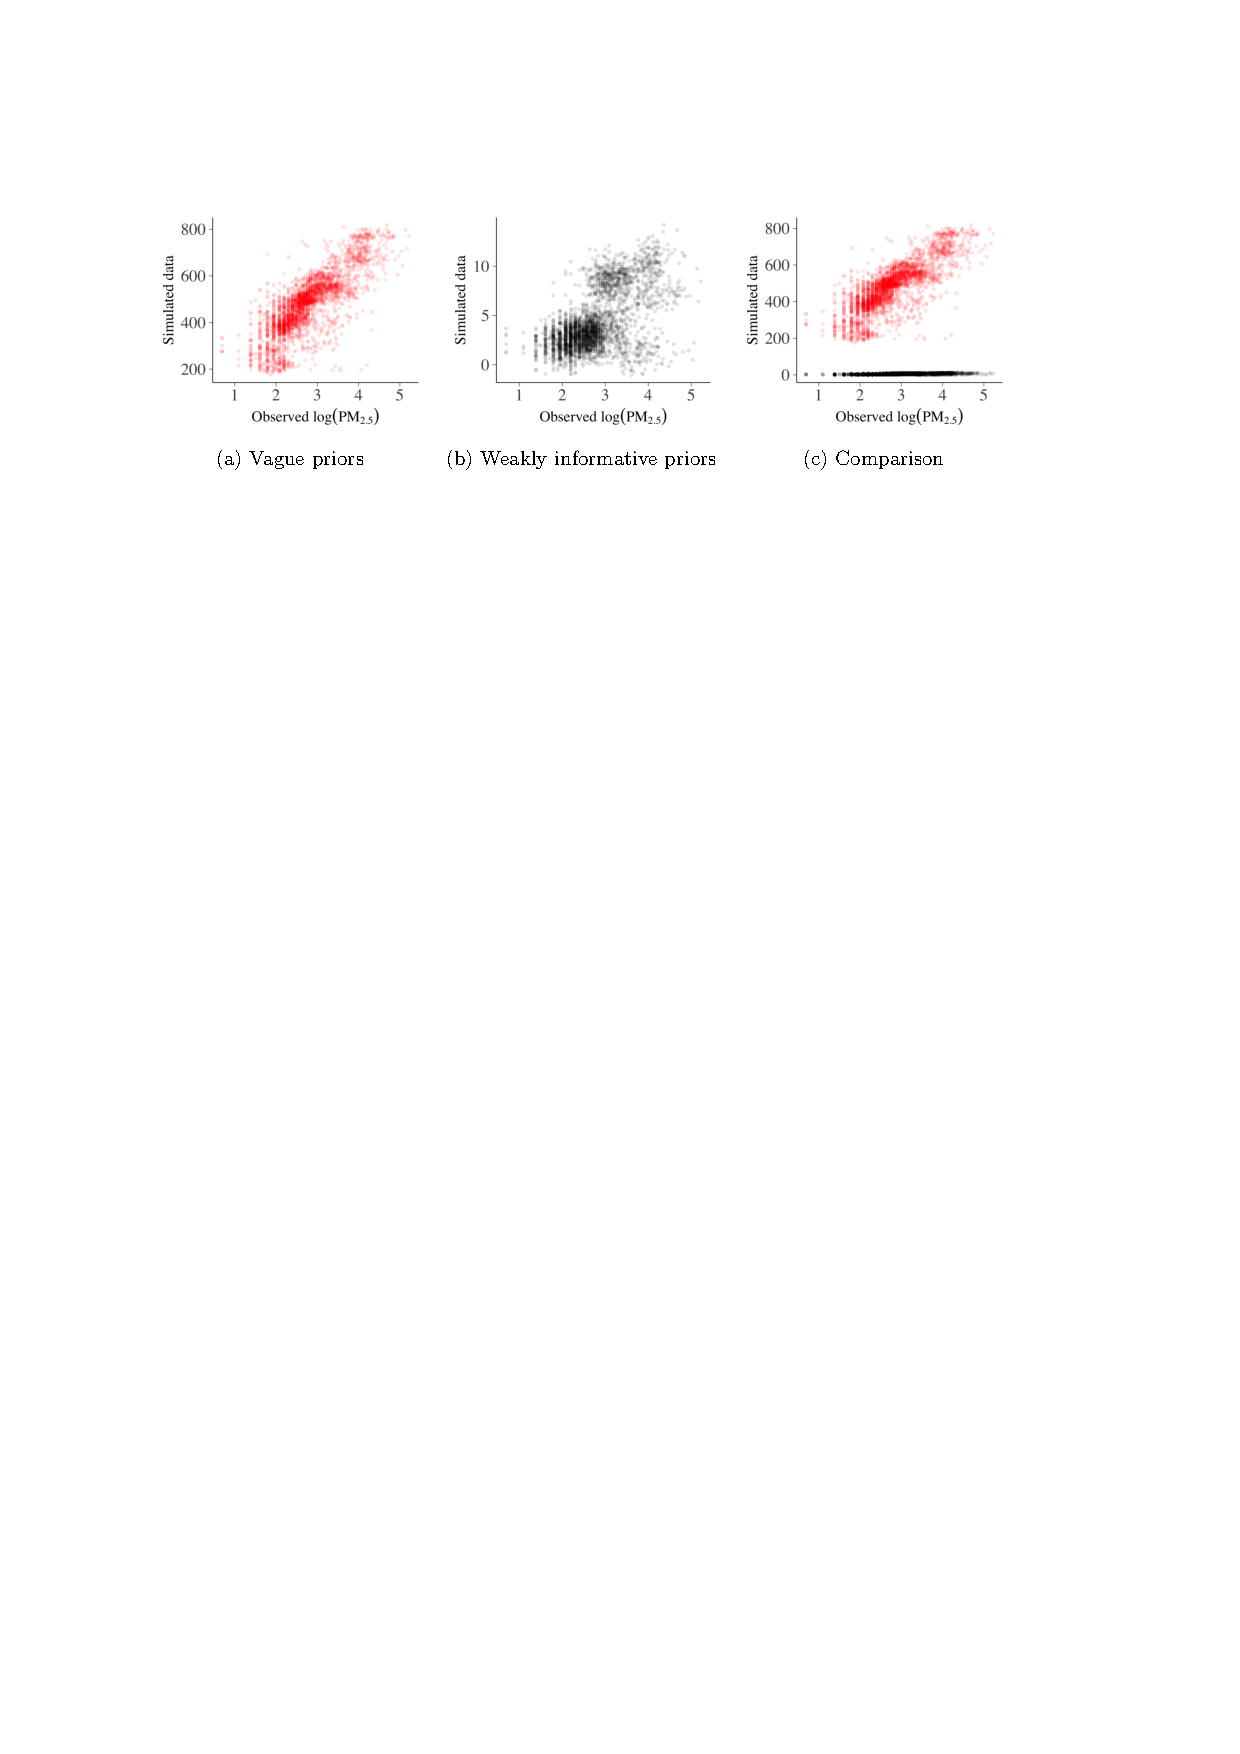
\includegraphics[width=0.9\textwidth]{img/prior-predictive-eg.pdf}
\end{center}
\vspace*{-10pt}
\begin{itemize}
\item \myemph{particulate matter pollution} model with prior on
  $\log(\textrm{PM}_{2.5})$
\item \myemph{vague prior} generates values as dense as neutron star
\item \myemph{weakly informative} prior controls scale
\item subtle with priors on \myemph{interacting parameters}
  \begin{subitemize}
  \item why we need a PPL!
  \end{subitemize}
\end{itemize}

\sld{How does Stan fare?}
\begin{itemize}
\item Stan model for \myemph{posterior inference}
\vspace*{-6pt}
{\footnotesize
\begin{verbatim}
  data { int<lower=0> N; int<lower=0, upper=1> y[N]; }
  parameters { real<lower=0, upper=1> theta; }
  model { theta ~ beta(2, 10);  y ~ binomial(theta); }
\end{verbatim}
}
\item Simulate $\simvar{\theta} \sim p(\theta)$ with $N = 0$, but
  \myemph{can't simulate} $y$!
\item Need \myemph{alternative Stan model} for \myemph{prior predictive checks}
\vspace*{-6pt}
{\footnotesize
\begin{verbatim}
  data { int N; }
  parameters { real<lower=0, upper=1> theta; }
  model { theta ~ beta(2, 10); }
  generated quantities { 
    int y_sim[N] = bernoulli_rng(N, theta);
  }
\end{verbatim}
}
\end{itemize}

\sld{How do other PPLs fare?}
\begin{itemize}
\item \myemph{PyMC} typically declares data but \myemph{doesn't have to}:
\vspace*{-6pt}
{\footnotesize 
\begin{verbatim}
    y_obs = pm.Normal("y_obs", mu=X @ weights, 
                      sigma=noise, observed=y) 
\end{verbatim}
\vspace*{-8pt}
}
\item \myemph{ADMB} declares data in a \myemph{\texttt{DATA SECTION}}
\item \myemph{Pyro} uses effect handler \myemph{\texttt{condition()}} for data, e.g., 
\vspace*{-6pt}
{\footnotesize 
\begin{verbatim}
    poutine.condition(model, data={"z": 1.0})
\end{verbatim}
\vspace*{-8pt}
}
\item \myemph{Turing.jl} assigns data variables before
  just-in-time compilation; values may be specified
  \myemph{\texttt{missing}}
\item \myemph{BUGS} sets data at run time w.r.t.\ its neutral graphical model
\vspace*{-12pt}
{\footnotesize 
\begin{verbatim}
  theta ~ dbeta(2, 10); for (n in 1:N) y[n] ~ dbern(theta); 
\end{verbatim}}
\end{itemize}


\sld{Simulation-based Calibration}
\begin{itemize}
\item to \myemph{validate inference} w.r.t.\ well-specified data
  \begin{subitemize}
    \item approximate inference like VI will fail
    \end{subitemize}
  \item draw $\simvar{\theta} \sim p(\theta)$ from the prior
  \item draw $\simvar{y} \sim p(y \mid \simvar{\theta})$ from the
    sampling distribution
  \item draw $\draw{\theta}{1}, \ldots, \draw{\theta}{M} \sim p(\theta
    \mid \simvar{y})$ from algorithm to test
  \item because $(\simvar{y}, \simvar{\theta}) \sim p(y, \theta)$ and
    $(\simvar{y}, \draw{\theta}{m}) \sim p(y, \theta)$,
    $\simvar{\theta}$ and the $\draw{\theta}{m}$
    should be \myemph{identically distributed}
  \item Allows a \myemph{statistical test} of uniformity w.
    marginal ranks.
    \vfill
    {\footnotesize Cook,  Gelman, Rubin.
      2006. Validation of software for Bayesian models using posterior
      quantiles. \textit{JCGS}.}
\end{itemize}

\sld{SBC diagnoses}
\begin{itemize}
  \item 
    \myemph{over-dispersed}: \hfill
    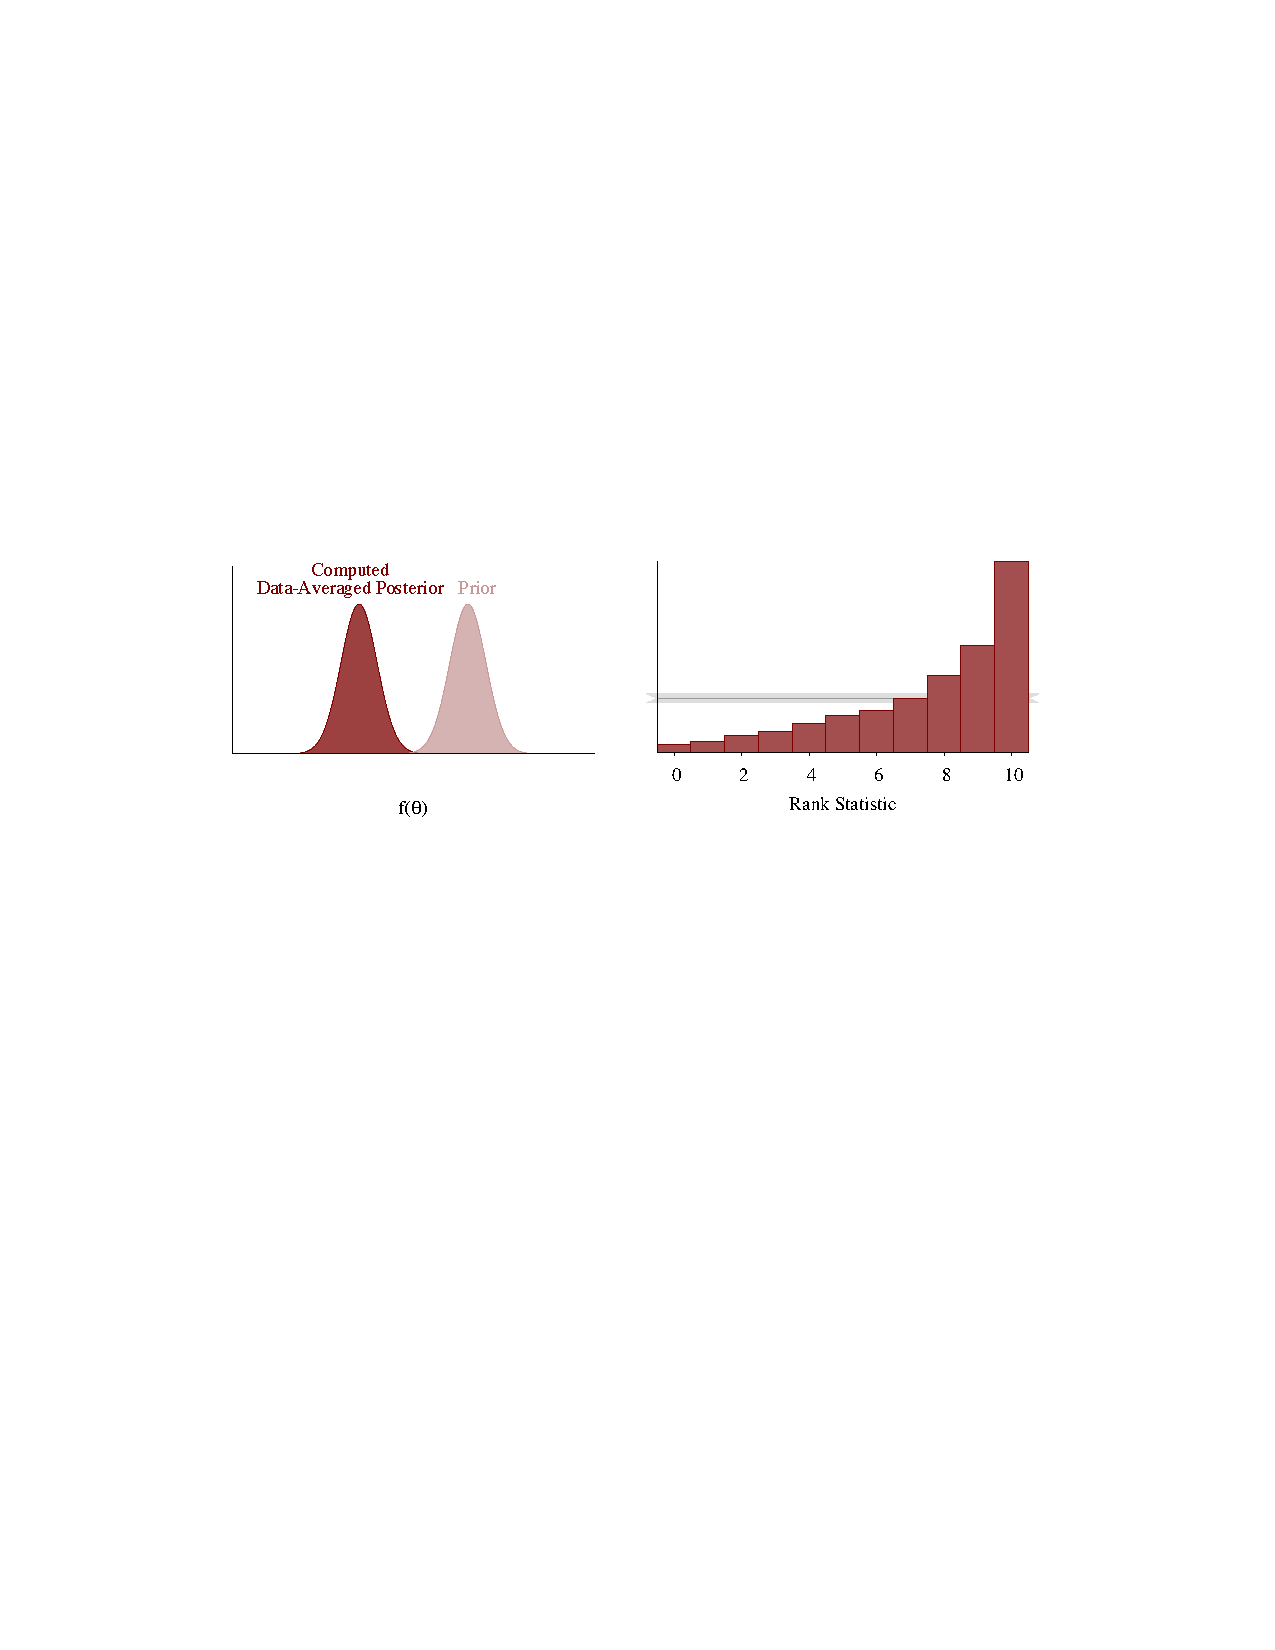
\includegraphics[valign=c,width=0.5\textwidth]{img/sbc-over.pdf}
  \item 
    \myemph{under-dispersed}: \hfill
    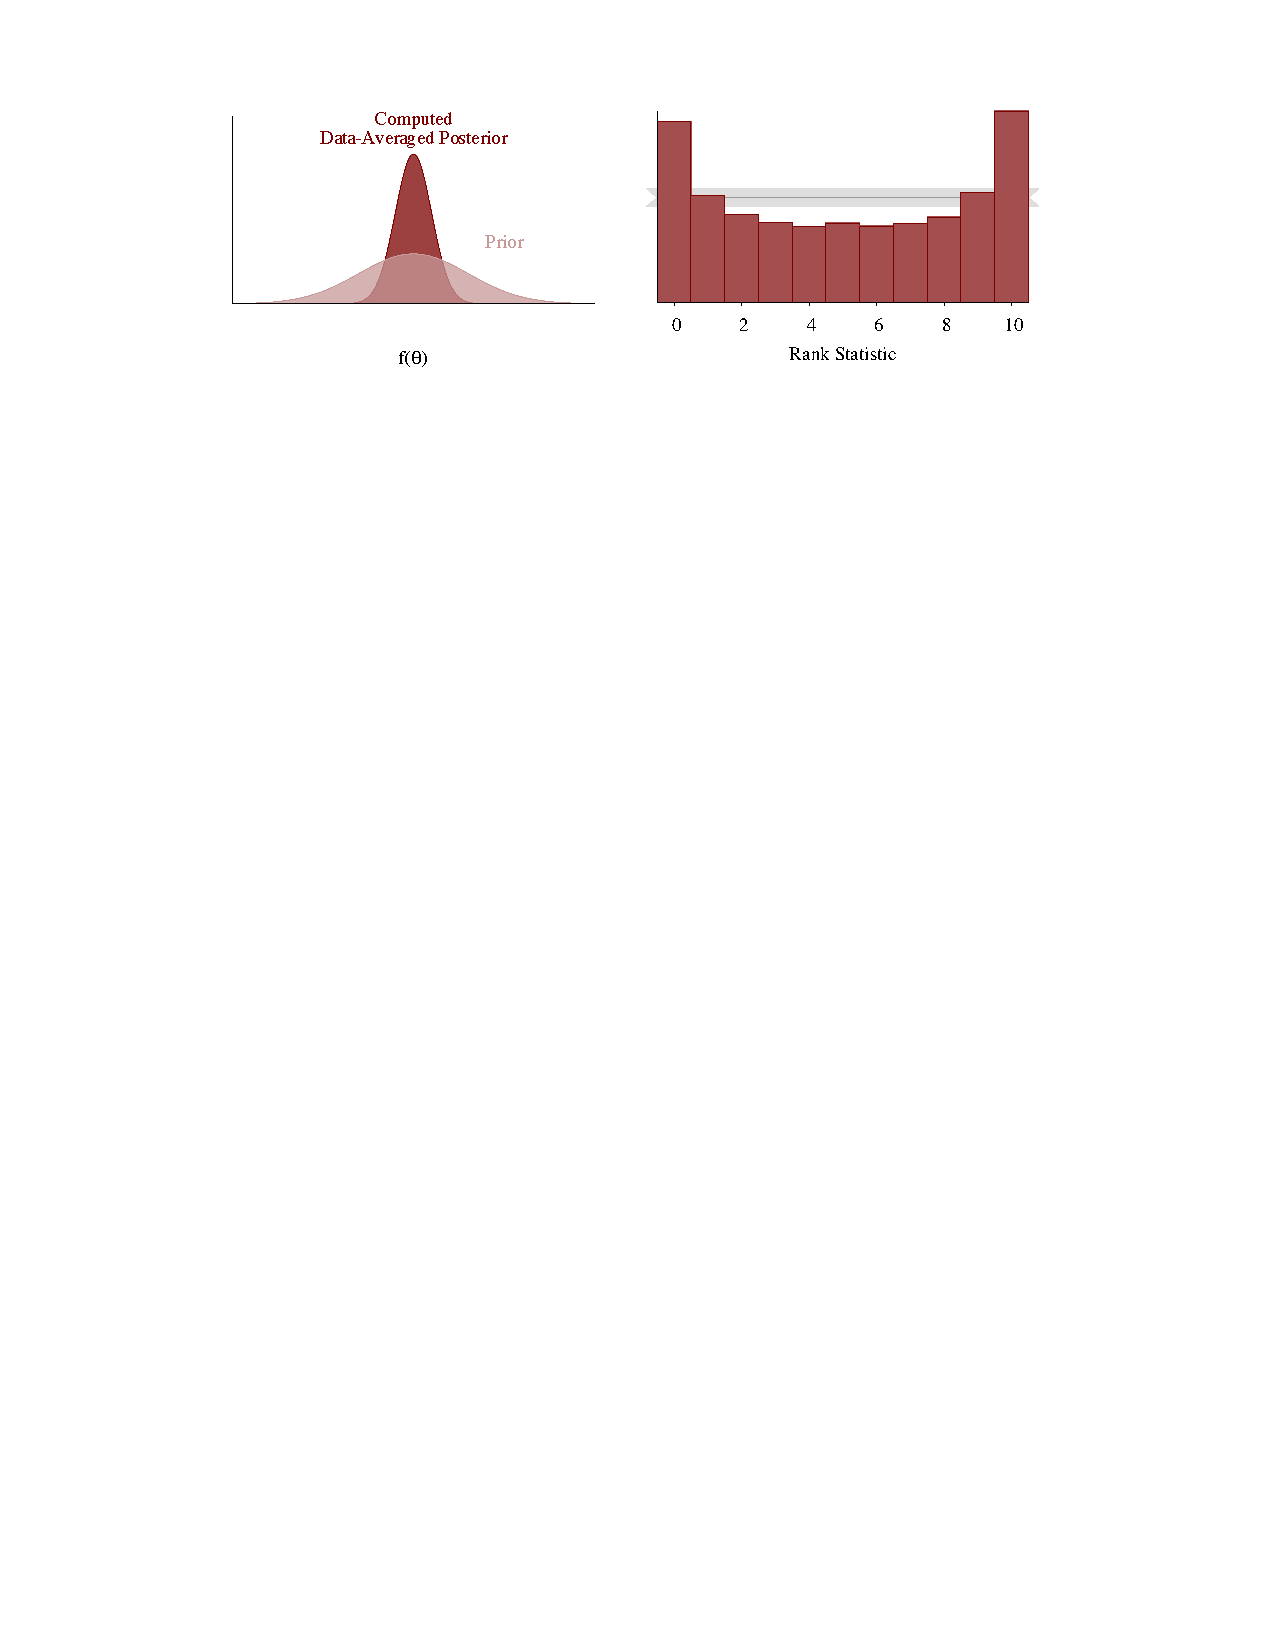
\includegraphics[valign=c,width=0.5\textwidth]{img/sbc-under.pdf}
  \item 
    \myemph{skewed}: \hfill
    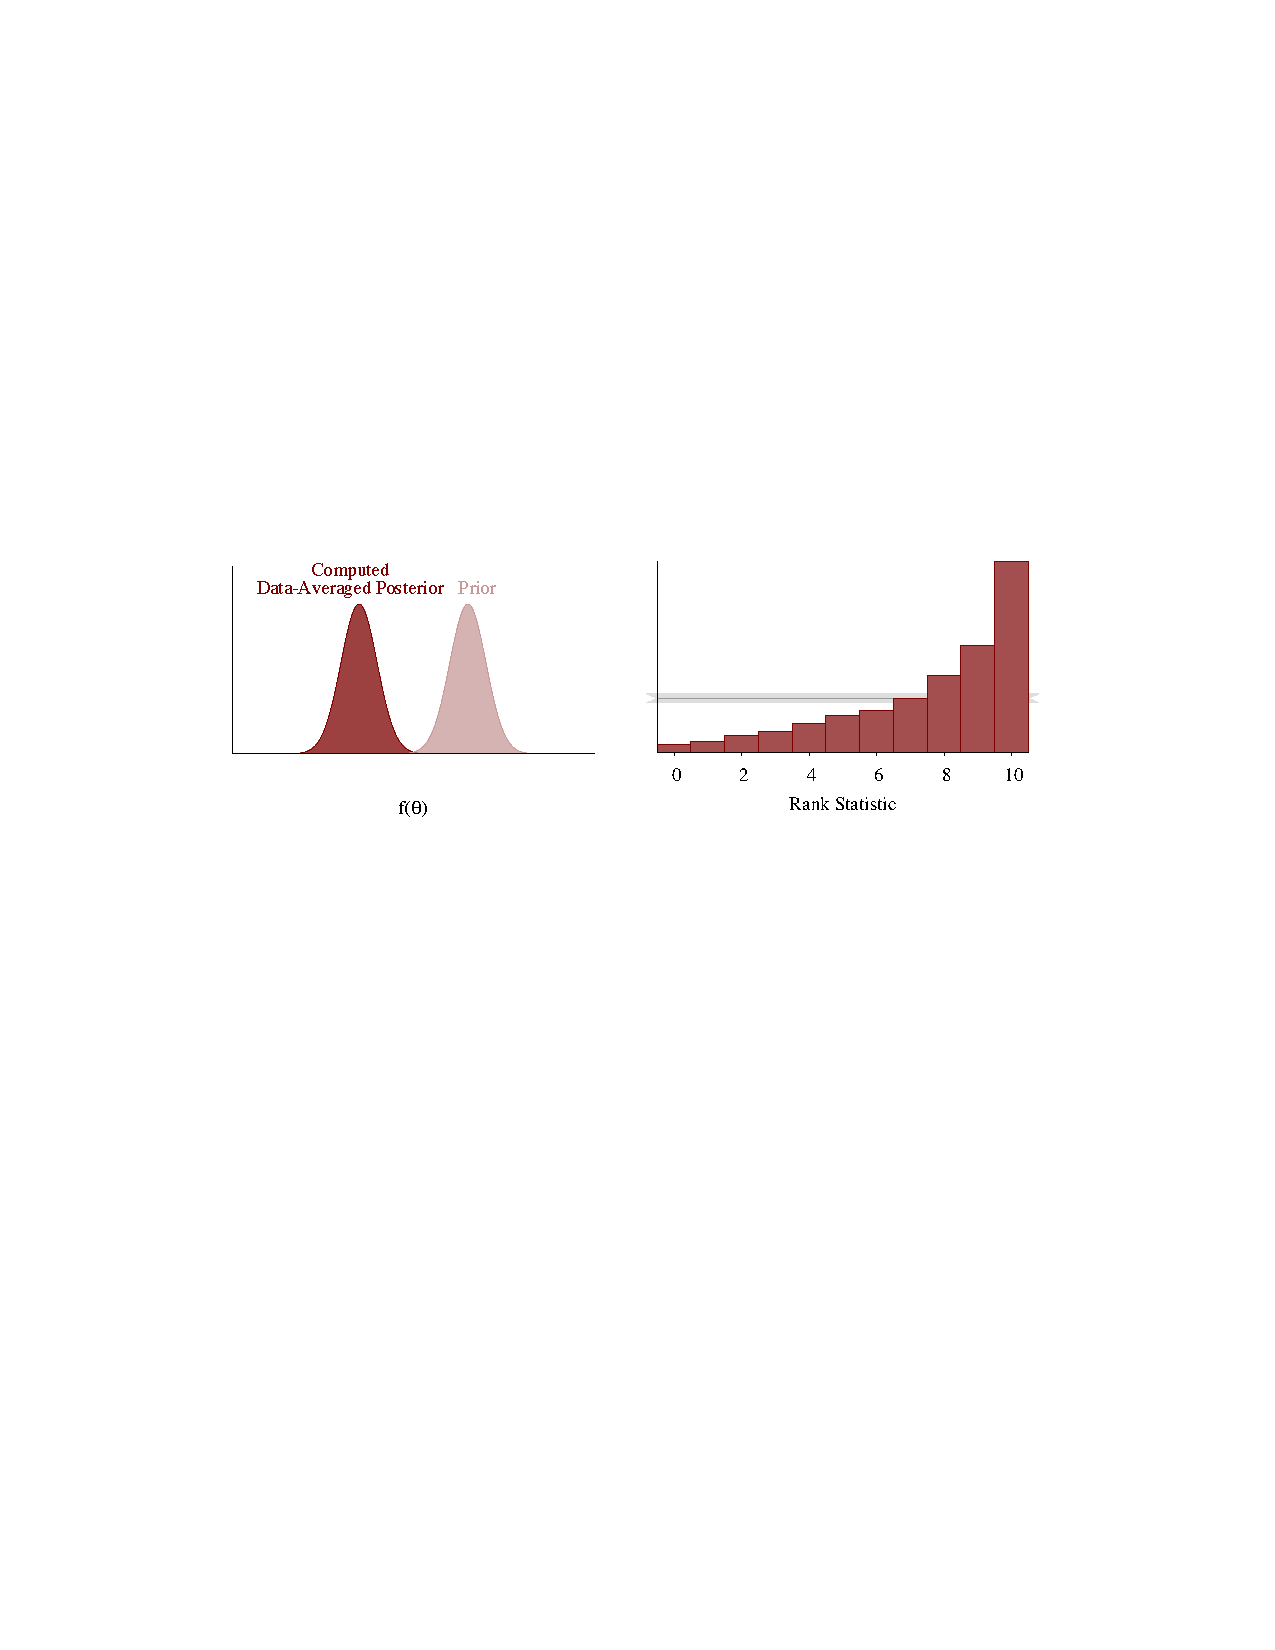
\includegraphics[valign=c,width=0.5\textwidth]{img/sbc-skew.pdf}
\end{itemize}



\sld{How do PPLs fare on SBC?}

\begin{itemize}
\item simulation-based calibration requires simulating from prior and
  sampling distribution
\item presents same problem with data specification as prior
  predictive checks
\end{itemize}

\sld{Posterior predictive checks}
\begin{itemize}
\item Simulate new data from posterior for draws $m \in 1{:}M$,
  \begin{eqnarray*}
    \draw{\theta}{m} & \sim & p(\theta \mid y)
    \\
    \simdraw{y}{m} & \sim & p(y \mid \draw{\theta}{m})
  \end{eqnarray*}
\item Compare statistics $s(y)$ on observed data to those
  of posterior simulations $s(\simdraw{y}{m})$, e.g.,
  \begin{subitemize}
  \item $s()$ can be anything, e.g., mean, max, sd, quantiles, ranks,
    skew, etc.
  \end{subitemize}
\item Plot, or compute two-sided posterior $p$-values to automate,
  \[
    p\textrm{-value} = \min(\begin{array}[t]{l}
                              \textrm{Pr}[s(y) < s(\simvar{y})],
                              \\[4pt]
                              1 - \textrm{Pr}[s(y) < s(\simvar{y})] \ )
                              \end{array}
  \]
\end{itemize}

\sld{Posterior predictive example}
\begin{center}
\vspace*{-10pt}
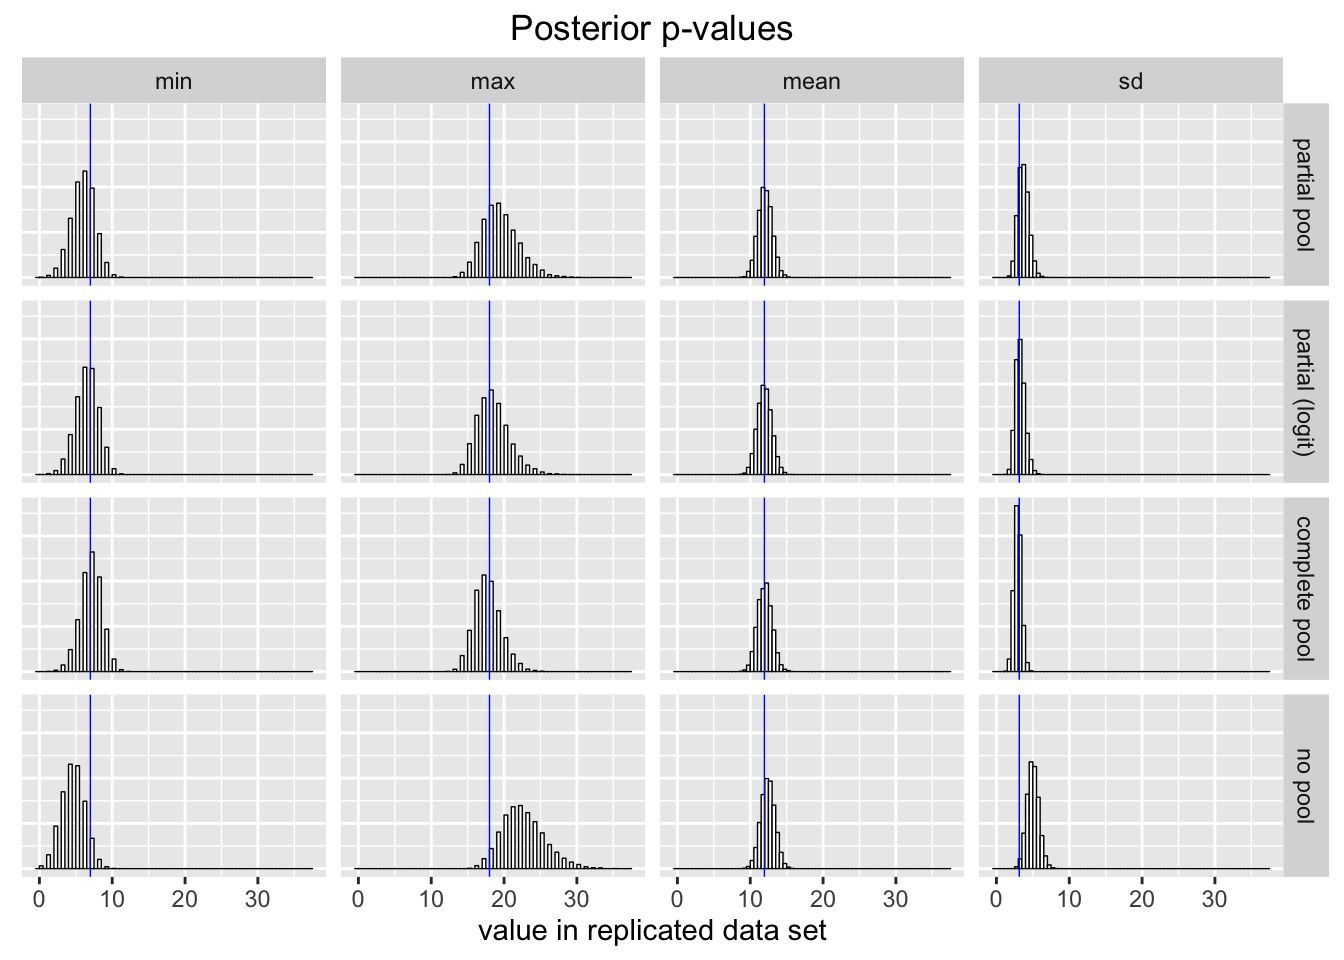
\includegraphics[width=0.6\textwidth]{img/ppc-binary-trials.png}
\vspace*{-10pt}
\end{center}
\begin{itemize}
\item model of repeated binary trials (baseball batting avg.)
  \begin{subitemize}
    \item vertical line is $s(y)$, histogram is $s(\simdraw{y}{m})$
    \item max() and sd() statistics ``reject'' the no-pooling model
  \end{subitemize}
\end{itemize}

\sld{PPL support for PPCs}
\begin{itemize}
\item requires extracting posterior draws and simulating data from
  them
\item still the same problem of flexibly specifying data
  vs.\ parameters (i.e., knowns vs.\ unknowns)
\end{itemize}

\sld{Cross-validation}
\begin{itemize}
\item divide data into train/test split (say $y$ and $\widetilde{y}$)
\item fit model on training set
\item evaluate predictive log density on test set,
  \begin{eqnarray*}
    \log p(\tilde{y} \mid y)
    & \approx & \log \frac{1}{M} \sum_{m=1}^M p(\tilde{y} \mid \simdraw{\theta}{m})
    \\[4pt]
    & = & \textrm{log-sum-exp}_{m=1}^M \, \log p(\tilde{y} \mid
          \simdraw{\theta}{m})
          - \log(M)
  \end{eqnarray*}
\end{itemize}

\sld{PPL support for X-val}
\begin{itemize}
\item fit with one data set $y$
  and evaluate with another $\tilde{y}$
\item \myemph{BUGS} almost succeeds
\vspace*{-8pt}
{\footnotesize 
\begin{verbatim}
  for (n in 1:N) y[n] ~ dnorm(alpha + x[n] * beta, tau)
  tau ~ gamma(1, 1);  alpha ~ normal(0, 2);  beta ~ normal(0, 2)
\end{verbatim}
\vspace*{-8pt}}
by letting $y = y^{\textrm{train}}, y^{\textrm{test}}$ be partially
missing
\begin{subitemize}
  \item but doesn't let you retrieve the log density values for $y^{\textrm{test}}$
\item this also seamlessly handles missing data (that's modeled)
\end{subitemize}
\item \myemph{Turing.jl} allows the same thing (values?)
\item other PPLs require additional sampling statements for the test data
\end{itemize}  

\sld{Stan for X-val}
\begin{itemize}
\item Stan codes \myemph{leave-one-out X-val} by specifying test point
\vspace*{-6pt}
{\footnotesize 
\begin{verbatim}
data { 
  int N; int[N] y;  int nt;
}
parameters { 
  real mu; real<lower=0> sigma;
}
model { 
  append_row(y[:nt-1], y[nt+1:]) ~ normal(mu, sigma);
  mu ~ normal(0, 1);  sigma ~ lognormal(0, 1);
}
generated quantities {
  real lp = normal_lpdf(y[nt] | mu, sigma);
}
\end{verbatim}
  \vspace*{-8pt}}
\item but it's a \myemph{totally different model}
\end{itemize}

\sld{Sensitivity analysis}
\begin{itemize}
\item we'd like to understand how \myemph{changes in our model affect
  posterior inference}
\item e.g., vary priors and see how posterior expectations changes
\item all PPLs let you evaluate alternative constants easily
\item \myemph{derivative-based sensitivity} w.r.t.\ const. $c$ is trickier
  \[
    \frac{\partial}{\partial c} \mathbb{E}[f(\theta) \mid y, c]
  \]
  Ryan Giordano modified Stan's C++ to compute this for his (Berkeley)
  Ph.D. thesis, but it's not exposed
\end{itemize}  

\sld{Sensitivity example}
\begin{center}
\vspace*{-10pt}
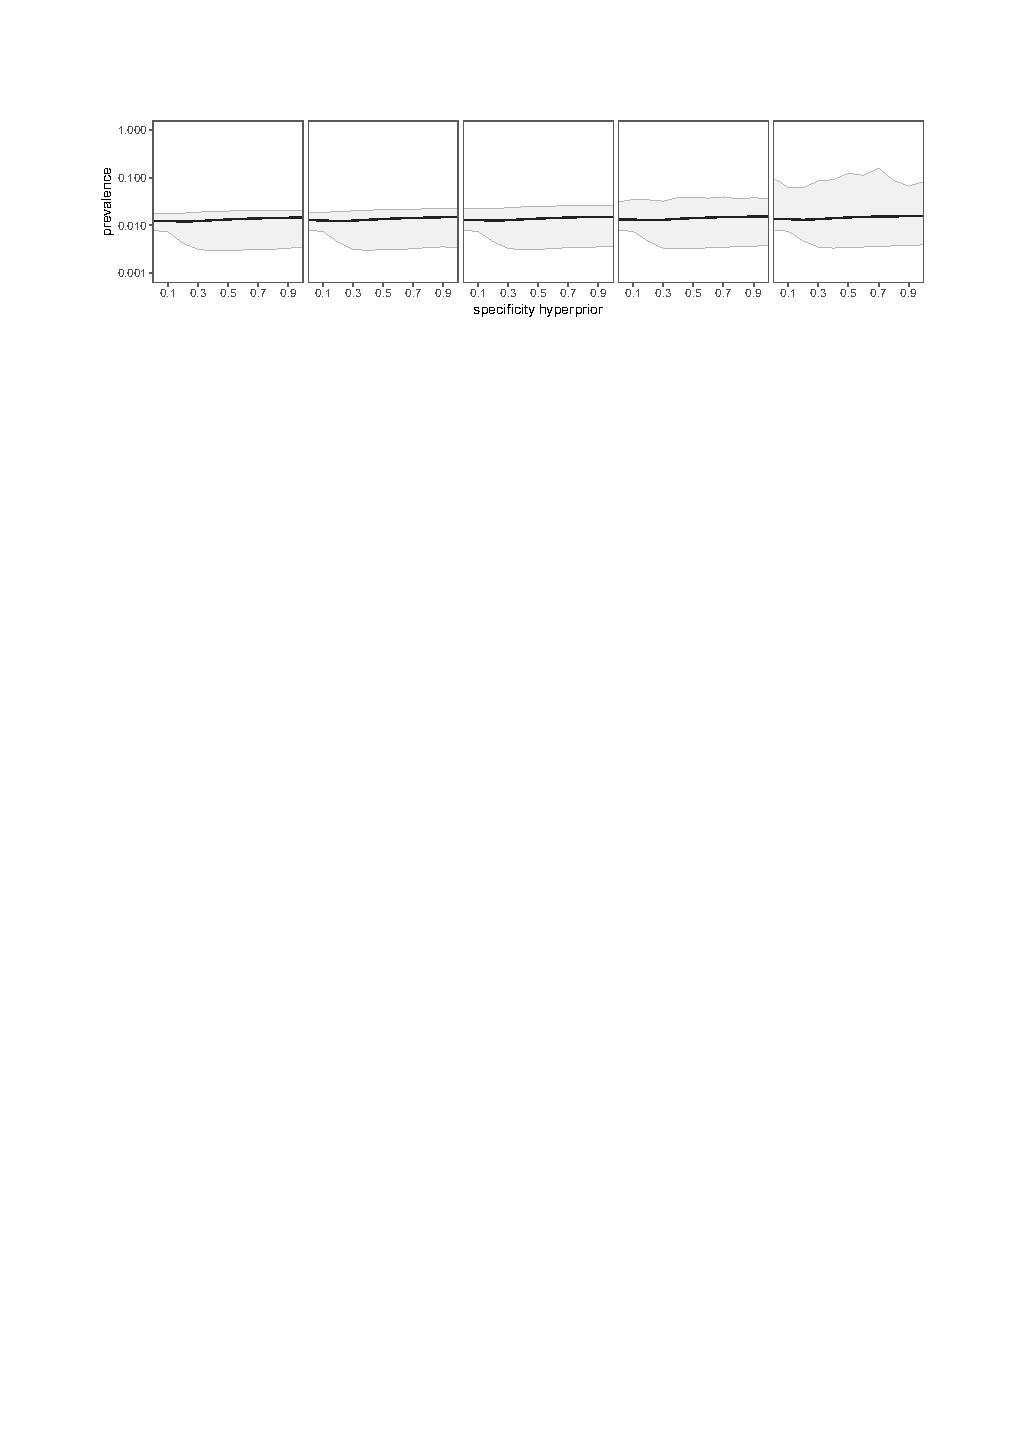
\includegraphics[width=0.9\textwidth]{img/covid-sensitivity.pdf}
\vspace*{-10pt}
\end{center}
\begin{itemize}
\item Estimated Covid seroprevalence ($y$ axis) as a function of
  \begin{subitemize}
  \item the hyperprior for specificity ($x$-axis)
  \item the hyperprior for sensitivity (facets with values from left-to-right
    0.01, 0.25, 0.5, 0.75, 1.0)
  \end{subitemize}
\vfill
{\footnotesize $\bullet$\
Gelman, Carpenter. 2020. Bayesian analysis of tests with unknown
specificity and sensitivity. \textit{JRSS C}.}
\end{itemize}

\sld{Workflow goes beyond inference}
\begin{itemize}
\item \myemph{clamp/pin parameters} to fixed values?
  \begin{subitemize}
    \item Stan requires moving the variable from the parameter to the
      data block
  \end{subitemize}
\item working with \myemph{multiple (related) models}?
  \begin{subitemize}
  \item model comparison
  \item model reparameterization
  \item model averaging/mixing/stacking
  \end{subitemize}
\item \myemph{autogenerating} concurrent or GPU code?
  \begin{subitemize}
    \item Stan requires using parallel map functions in the program
  \end{subitemize}`
\end{itemize}

\sld{Naming and persistence is hard}
\begin{itemize}
\item how to \myemph{name and store multiple model variants}?
  \begin{subitemize}
    \item \texttt{uk-covid-icar}, \texttt{uk-covid-rw1}, \\
      \texttt{uk-covid-rw2}, \texttt{uk-covid-rw2-icar}, \\
      \texttt{uk-covid-rw2-bym2}, \texttt{uk-covid-rw2-bym2pc}, \\
      \texttt{uk-covid-rw2-bym2pc-no-socio},
      \textit{ad infinitum} $\ldots$
    \item plus multiple versions of the same model (over time)
  \end{subitemize}
\item how to \myemph{name and store output}?
\item how to work with \myemph{distributed teams}?
  \begin{subitemize}
  \item e.g., how to \myemph{share results} given that samples can be
    large?
  \item or that they run on clusters in pieces
  \end{subitemize}
\end{itemize}

\sld{Other workflow issues}
\begin{itemize}
\item data may be tied up with \myemph{privacy} and/or \myemph{intellectual property}
  concerns
  \begin{subitemize}
  \item e.g., medical records, search logs, street views, etc.
  \end{subitemize}
\item end application may require \myemph{deployment in production}
  \begin{subitemize}
  \item bundle with Docker, or otherwise deploy
  \item robustness is a key issue
  \item update as new data comes in
  \end{subitemize}
  \vfill
  \item \myemph{What are we missing?}
\end{itemize}

\sld{Democratization of modeling}
\begin{itemize}
\item \myemph{expression-based iterfaces} use PPLs under the hood, but
  give users simpler specification sublanguages
  \begin{subitemize}
  \item \myemph{brms}: expression interface in R
  \item a Poisson GLM with log link is a one-liner
\begin{verbatim}
  y ~ age + base * treatment + (1 | patient)
\end{verbatim}
    \end{subitemize}
\item \myemph{fully encapsulated interfaces} use PPLs under the hood
  but give users a menu of model choices
  \begin{subitemize}
    \item \myemph{Prophet} (time-series with trends and cycles)
    \item \myemph{Torsten} (PK/PD compartment models)
    \end{subitemize}
  \item these systems involve \myemph{lots of defaults}
    \begin{subitemize}
      \item \myemph{evaluation crosses application boundaries}
      \end{subitemize}
    \end{itemize}

\sld{Elephant in the room: Modularity}
\begin{itemize}
\item how to \myemph{modularize model components} like hierarchical
  priors or GP priors?
\item Stan lets users define \myemph{functions}
  \begin{subitemize}
  \item e.g., a random-walk or ICAR prior's density function
  \end{subitemize}
\item but they \myemph{can't cross block boundaries}, e.g., 
  data, parameter, model, generated quantities
\item what about other PPLs?
  \vfill
\item a residual problem: \myemph{density is modular, behavior isn't}
  \begin{subitemize}
    \item e.g., a prior can only be understood in the context of a
      likelihood and a data set
  \end{subitemize}
\end{itemize}

\sld{References}
\begin{itemize}
\item \myemph{workflow paper}
  \begin{subitemize}
    \item Gelman, Vehtari, Simpson, Margossian, Carpenter, Yao, Kennedy,
    Gabry, Bürkner, Modrák. 2020. Bayesian workflow. \textit{arXiv}.
  \end{subitemize}
\item open-access \myemph{workflow book}
  \begin{subitemize}
  \item Above authors give or take. 2025(?) \textit{Bayesian Workflow}. Chapman \& Hall/CRC.
  \item GitHub repo: \\ {\small \url{https://github.com/jgabry/bayes-workflow-book}}
  \end{subitemize}
\end{itemize}
  

\end{document}

\vspace*{-6pt}
{\footnotesize 
\begin{verbatim}
\end{verbatim}
\vspace*{-8pt}}

\item \footnotesize Gelman, Vehtari, Simpson, Margossian, Carpenter, 
    Yao, Kennedy, Gabry, Bürkner, and Modrák. 2020. \myemph{Bayesian workflow}. 
    \textit{arXiv} 2011.01808.
  \item Book draft:
    \url{https://github.com/jgabry/bayes-workflow-book}

    \sld{Workflow's more than inference!}
\begin{center}
\vspace*{-6pt}
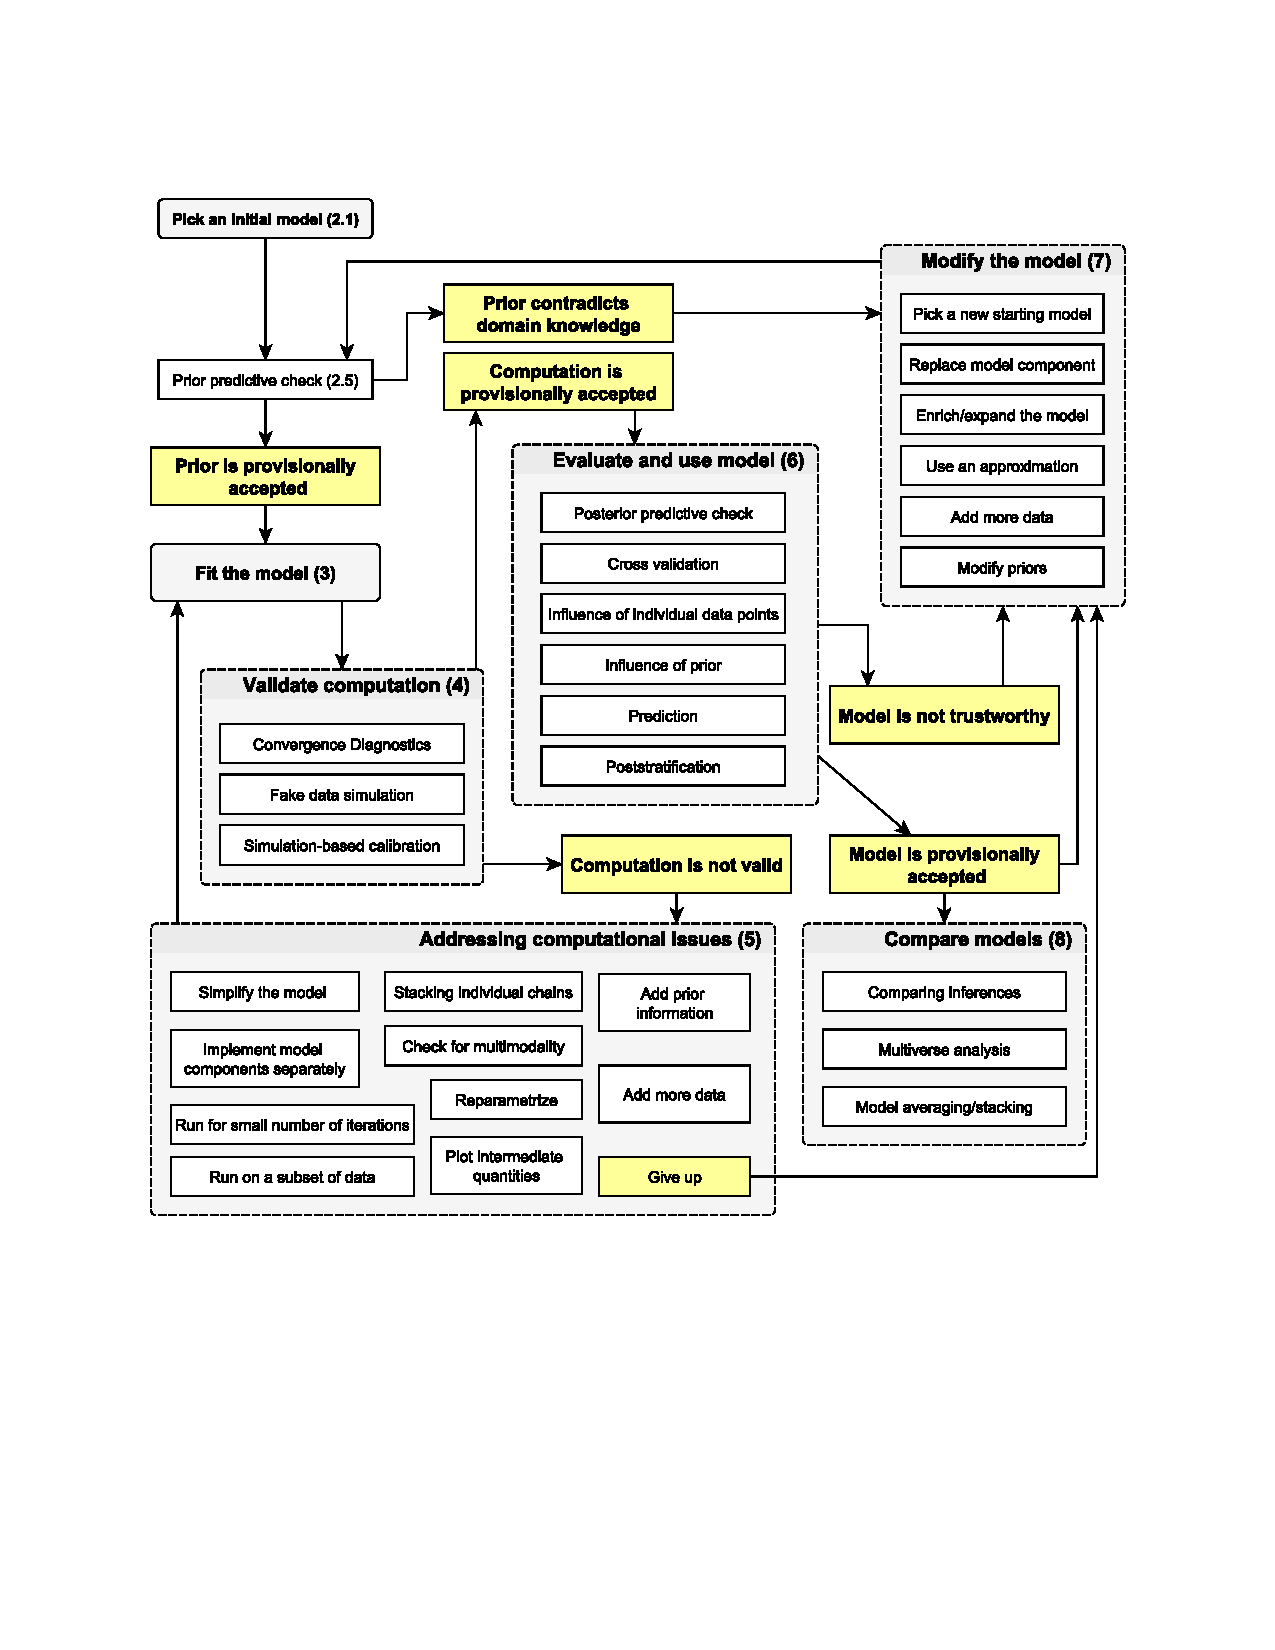
\includegraphics[height=0.7\textheight]{img/workflow-fig.pdf}
\end{center}
\begin{itemize}
\item where else might PPLs help? 
\end{itemize}

